%%% -*- TeX-master: "../main" -*-
\chapter{Dynamic Vision Sensor}
\label{cha:dvs}

In \citeyear{dvs} \citeauthor{dvs} proposed the design for the asynchronous
temporal contrast vision sensor, a neuromorphic, frame-free image sensor. Later
a spin-off company called inilabs built this design into the dynamic vision
sensor (DVS) which they distribute to labs around the world as part of their
neuromorphic product suite. Additionally, they develop the software jAER for
recording, replaying and manipulating DVS data.

The DVS produces a stream of illumination change events whereas a pixel
generates an event as soon as it detects a change in illumination that exceeds a
configurable threshold without synchronization with surrounding pixels. It is
this property that makes the sensor comparable to ganglion cells in the human
retina insofar as the pixels act asynchronously and react to illuminance changes
over time. As a consequence, under constant lighting conditions, the sensor
captures most of its signal at the edges of objects because smooth surfaces such
as human skin have almost constant illumination when moving in front of the DVS.
So, opposed to conventional cameras that transmit the whole picture with each
frame, the DVS filters out redundant information from still standing objects
which thus incur neither transmission nor computational costs. Therefore the DVS
lends itself particularly well to applications that run on battery or have to
rely on low-power microcontrollers such as aerial drones. Another proposed
application are surveillance scenarios, for example traffic monitoring or
security cameras, that primarily detect movement and track objects in video
streams and thus could run on cheaper hardware if the vision sensor would filter
out movement from the beginning. Finally, the DVS does not exhibit motion blur
because each pixel generates an event as soon as a change in illumination is
registered. This makes it a good fit for tracking fast moving objects, for
example in robotics or human-computer interfaces such as eye trackers or gesture
recognition. Furthermore, the device has already been used to track the wings of
fruit flies and particles in fluid dynamics experiments.

The sensor has a spatial resolution of 128$\times$128 pixels and a temporal
resolution of \SI{10}{\micro\second}. This means that events are timestamped by
a free-running counter ticking up at \SI{100}{\kilo\hertz}. Due to the DVS being
a CMOS chip, it just consumes \SI{23}{\milli\watt} of power. Each pixel has a
logarithmic photoreceptor circuit which lets the DVS operate over a dynamic
range of \SI{120}{\decibel}. Formally, each pixel circuit tracks the temporal
contrast defined as $c = \nicefrac{\mathrm{d}}{\mathrm{d}t} \log I$, i.e. it is
the gradient of the log-intensity of the incoming light. An event is triggered
whenever the temporal contrast exceeds a threshold in either direction, i.e. $c
< \theta_{\mathrm{off}}$ or $c > \theta_{\mathrm{on}}$. The former condition
generates an OFF event while the latter generates an ON event. The type of an
event is also called the polarity and is defined as the sign of the temporal
contrast that triggered it, $p = \mathrm{sign}(c)$. The whole process has a
latency of \SI{15}{\micro\second} and activates a reset transistor that imposes
a refractory period on the pixel during which it cannot activate again. This
ensures fairness between pixels because in its absence a handful of pixels could
saturate the communication bus that is limited to about \SI{200}{keps} (kilo
events per second) without timestamping and \SI{60}{keps} with.

\begin{figure}
  \centering
  \begin{bytefield}[bitwidth=1.15em]{32}
    \bitheader[endianness=big]{0-31} \\
    \bitbox{16}{$t$} \bitbox{1}{} \bitbox{7}{$y$} \bitbox{7}{$x$} \bitbox{1}{$p$}
  \end{bytefield}
  \caption{Binary format of an address event}
  \label{fig:dvs:bytefield}
\end{figure}

The DVS streams events over USB in address-event representation (AER). In AER
each event is a 4-tuple $(t, x, y, p)$ where $t$ is the timestamp, $x$ and $y$
are the coordinates of the event's origin and $p$ is the event's polarity. On
the wire each tuple is encoded in \SI{4}{bytes} as shown in Figure
\ref{fig:dvs:bytefield}. The polarity is binary and can be encoded in a single
bit. The coordinates range from $0$ to $127$, thus they can be encoded in $7$
bits each since $2^{7} = 128$. Interestingly, $t$ is encoded as a \SI{16}{bit}
integer with a maximum value of $2^{16} - 1 = 65535$, even though it is
incremented $100,000$ times per second. Consequently, it wraps around up to two
times per second. jAER accounts for this by checking for wrap-around and
incrementing a separate \SI{32}{bit} counter accordingly.

\begin{figure}
  \centering
  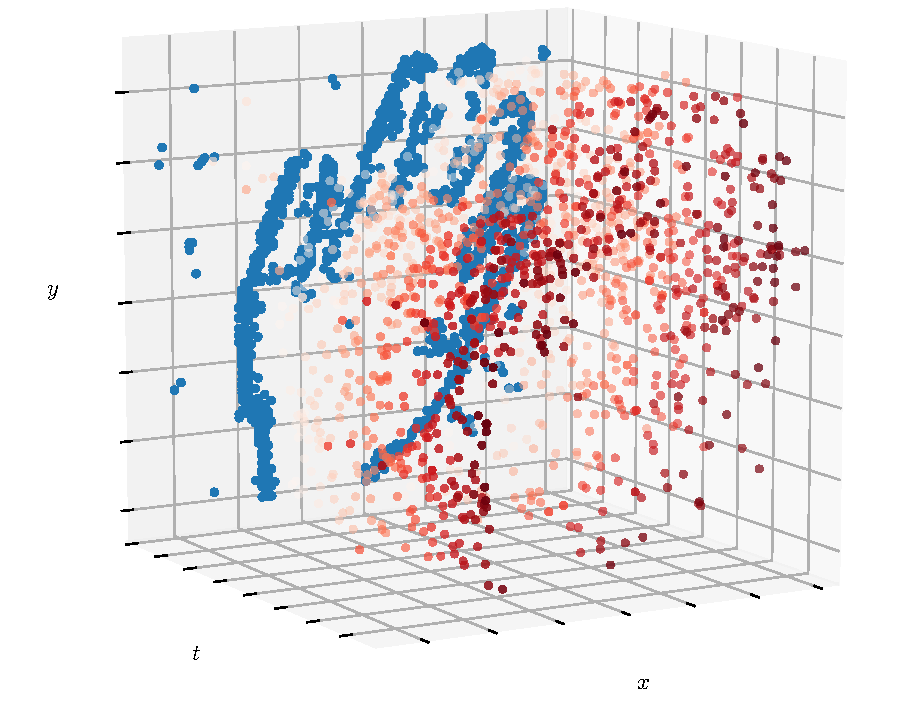
\includegraphics{figures/dvs/hand}
  \caption{Scatter plot of $1409$ events in a \SI{6.5}{\milli\second} long
    segment of a hand moving towards the sensor. The brightness of the red
    points indicates their timestamp $t$ while the blue points are a projection
    of the events onto the $x$-$y$-plane.}
  \label{fig:dvs:hand}
\end{figure}

There is another interpretation of event streams that is different from the
physical one introduced in this chapter. Figure \ref{fig:dvs:hand} shows a
\SI{6.5}{\milli\second} segment from a DVS recording of a hand moving towards
the sensor. You can interpret it as the hand moving through this $t$-$x$-$y$
space while the DVS samples points from the surface defined by the hand's
trajectory. We had originally hoped that this visualization would reveal a
tube-like structure through time. However, the samples from the trajectory
surface are too sparse for our vision to deduce the tubular shape and therefore
we added a projection of the data onto the $x$-$y$ plane in blue. Without this
visual aid, it would be difficult to make out the shape of the moving hand at
all.
